\documentclass[11pt,preprint, authoryear]{elsarticle}

\usepackage{lmodern}
%%%% My spacing
\usepackage{setspace}
\setstretch{1.2}
\DeclareMathSizes{12}{14}{10}{10}

% Wrap around which gives all figures included the [H] command, or places it "here". This can be tedious to code in Rmarkdown.
\usepackage{float}
\let\origfigure\figure
\let\endorigfigure\endfigure
\renewenvironment{figure}[1][2] {
    \expandafter\origfigure\expandafter[H]
} {
    \endorigfigure
}

\let\origtable\table
\let\endorigtable\endtable
\renewenvironment{table}[1][2] {
    \expandafter\origtable\expandafter[H]
} {
    \endorigtable
}


\usepackage{ifxetex,ifluatex}
\usepackage{fixltx2e} % provides \textsubscript
\ifnum 0\ifxetex 1\fi\ifluatex 1\fi=0 % if pdftex
  \usepackage[T1]{fontenc}
  \usepackage[utf8]{inputenc}
\else % if luatex or xelatex
  \ifxetex
    \usepackage{mathspec}
    \usepackage{xltxtra,xunicode}
  \else
    \usepackage{fontspec}
  \fi
  \defaultfontfeatures{Mapping=tex-text,Scale=MatchLowercase}
  \newcommand{\euro}{€}
\fi

\usepackage{amssymb, amsmath, amsthm, amsfonts}

\def\bibsection{\section*{References}} %%% Make "References" appear before bibliography


\usepackage[round]{natbib}

\usepackage{longtable}
\usepackage[margin=2.3cm,bottom=2cm,top=2.5cm, includefoot]{geometry}
\usepackage{fancyhdr}
\usepackage[bottom, hang, flushmargin]{footmisc}
\usepackage{graphicx}
\numberwithin{equation}{section}
\numberwithin{figure}{section}
\numberwithin{table}{section}
\setlength{\parindent}{0cm}
\setlength{\parskip}{1.3ex plus 0.5ex minus 0.3ex}
\usepackage{textcomp}
\renewcommand{\headrulewidth}{0.2pt}
\renewcommand{\footrulewidth}{0.3pt}

\usepackage{array}
\newcolumntype{x}[1]{>{\centering\arraybackslash\hspace{0pt}}p{#1}}

%%%%  Remove the "preprint submitted to" part. Don't worry about this either, it just looks better without it:
\makeatletter
\def\ps@pprintTitle{%
  \let\@oddhead\@empty
  \let\@evenhead\@empty
  \let\@oddfoot\@empty
  \let\@evenfoot\@oddfoot
}
\makeatother

 \def\tightlist{} % This allows for subbullets!

\usepackage{hyperref}
\hypersetup{breaklinks=true,
            bookmarks=true,
            colorlinks=true,
            citecolor=blue,
            urlcolor=blue,
            linkcolor=blue,
            pdfborder={0 0 0}}


% The following packages allow huxtable to work:
\usepackage{siunitx}
\usepackage{multirow}
\usepackage{hhline}
\usepackage{calc}
\usepackage{tabularx}
\usepackage{booktabs}
\usepackage{caption}


\newenvironment{columns}[1][]{}{}

\newenvironment{column}[1]{\begin{minipage}{#1}\ignorespaces}{%
\end{minipage}
\ifhmode\unskip\fi
\aftergroup\useignorespacesandallpars}

\def\useignorespacesandallpars#1\ignorespaces\fi{%
#1\fi\ignorespacesandallpars}

\makeatletter
\def\ignorespacesandallpars{%
  \@ifnextchar\par
    {\expandafter\ignorespacesandallpars\@gobble}%
    {}%
}
\makeatother

\newlength{\cslhangindent}
\setlength{\cslhangindent}{1.5em}
\newenvironment{CSLReferences}%
  {\setlength{\parindent}{0pt}%
  \everypar{\setlength{\hangindent}{\cslhangindent}}\ignorespaces}%
  {\par}


\urlstyle{same}  % don't use monospace font for urls
\setlength{\parindent}{0pt}
\setlength{\parskip}{6pt plus 2pt minus 1pt}
\setlength{\emergencystretch}{3em}  % prevent overfull lines
\setcounter{secnumdepth}{5}

%%% Use protect on footnotes to avoid problems with footnotes in titles
\let\rmarkdownfootnote\footnote%
\def\footnote{\protect\rmarkdownfootnote}
\IfFileExists{upquote.sty}{\usepackage{upquote}}{}

%%% Include extra packages specified by user
\usepackage{booktabs}
\usepackage{longtable}
\usepackage{array}
\usepackage{multirow}
\usepackage{wrapfig}
\usepackage{float}
\usepackage{colortbl}
\usepackage{pdflscape}
\usepackage{tabu}
\usepackage{threeparttable}
\usepackage{threeparttablex}
\usepackage[normalem]{ulem}
\usepackage{makecell}
\usepackage{xcolor}

%%% Hard setting column skips for reports - this ensures greater consistency and control over the length settings in the document.
%% page layout
%% paragraphs
\setlength{\baselineskip}{12pt plus 0pt minus 0pt}
\setlength{\parskip}{12pt plus 0pt minus 0pt}
\setlength{\parindent}{0pt plus 0pt minus 0pt}
%% floats
\setlength{\floatsep}{12pt plus 0 pt minus 0pt}
\setlength{\textfloatsep}{20pt plus 0pt minus 0pt}
\setlength{\intextsep}{14pt plus 0pt minus 0pt}
\setlength{\dbltextfloatsep}{20pt plus 0pt minus 0pt}
\setlength{\dblfloatsep}{14pt plus 0pt minus 0pt}
%% maths
\setlength{\abovedisplayskip}{12pt plus 0pt minus 0pt}
\setlength{\belowdisplayskip}{12pt plus 0pt minus 0pt}
%% lists
\setlength{\topsep}{10pt plus 0pt minus 0pt}
\setlength{\partopsep}{3pt plus 0pt minus 0pt}
\setlength{\itemsep}{5pt plus 0pt minus 0pt}
\setlength{\labelsep}{8mm plus 0mm minus 0mm}
\setlength{\parsep}{\the\parskip}
\setlength{\listparindent}{\the\parindent}
%% verbatim
\setlength{\fboxsep}{5pt plus 0pt minus 0pt}



\begin{document}



\begin{frontmatter}  %

\title{Modelling South African Salaries}

% Set to FALSE if wanting to remove title (for submission)




\author[Add1]{Emma Terblanche}
\ead{21777039@sun.ac.za}





\address[Add1]{Stellenbosch University}



\vspace{1cm}


\begin{keyword}
\footnotesize{
Machine Learning \sep Regularised Regressions \sep Linear Regressions \\
\vspace{0.3cm}
}
\end{keyword}



\vspace{0.5cm}

\end{frontmatter}


\renewcommand{\contentsname}{Table of Contents}
{\tableofcontents}

%________________________
% Header and Footers
%%%%%%%%%%%%%%%%%%%%%%%%%%%%%%%%%
\pagestyle{fancy}
\chead{}
\rhead{}
\lfoot{}
\rfoot{\footnotesize Page \thepage}
\lhead{}
%\rfoot{\footnotesize Page \thepage } % "e.g. Page 2"
\cfoot{}

%\setlength\headheight{30pt}
%%%%%%%%%%%%%%%%%%%%%%%%%%%%%%%%%
%________________________

\headsep 35pt % So that header does not go over title




\newpage

\hypertarget{introduction}{%
\section{Introduction}\label{introduction}}

With large scale poverty and unemployment levels, modelling South
African incomes is a vital part of performing economic analysis within
the South African context. There are multiple factors impacting a South
African's salary. Determining what these are and how they affect
someone's socioeconomic status allows for policy implementation to be
better targeted at improving standards of living. Fortunately, survey
datasets provide information on many possible influences. Machine
learning techniques are often used to more accurately conduct such
statistical analyses by providing methods to manage such an abundance of
features.

This paper compares the prediction ability of different machine learning
models on the monthly salaries of South Africans using the General
Household Survey (GHS) data of 2016. It trains five models, three of
which are linear regressions, and two are regularised regressions. The
linear regression methods used are multivariate linear regression,
principal component regression, and partial least squares regression.
Ridge regression and lasso regression are the two regularised regression
techniques used. The comparison metrics are Root Mean Squared Error
(RMSE) and R-squared. A model with a lower RMSE and a higher R-squared
is perceived to model salaries more accurately.

The Methodology section provides insight into the data cleaning and
manipulation techniques used prior to machine learning analysis. The
Results section explains each model used, as well as their RMSE and
R-squared scores. It also presents the features that each model deemed
most influential to South African salaries. The Discussion section draws
a comparison of the results. This paper concludes that the lasso
regression model performs marginally better than its counterparts.

\hypertarget{methodology}{%
\section{Methodology}\label{methodology}}

\hypertarget{data-and-manipulations}{%
\subsection{Data and Manipulations}\label{data-and-manipulations}}

The original GHS 2016 data set consists of 486 features with 75 972
observations. As this paper aims to model South African salaries, the
data set was restricted to include only the working age population. A
manipulated version of monthly salary is used as the dependent variable
in all five models. While there were no missing values in the data set,
the monthly salary feature contained two categories, ``Not Applicable''
and ``Unspecified'', that challenged its status as a numeric variable
which is needed for the modelling methods used. Those with
``Unspecified'' listed as their monthly salary were dropped from the
data, as they did not appear many times. The ``Not Applicable''
observations were changed to zero due to most of these individuals also
being unemployed, implying that they do not earn a salary. In order to
prevent the possibility of multicollinearity in the models, the other
income classification features, such as total income, were excluded.
After these changes, the final data set consisted of 469 variables with
43 450 observations. Furthermore, regularised regression requires all
dependent features to be numeric (Boehmke \& Greenwell, 2020). As the
caret-package is used, however, conversions of variables are done
automatically.

The resulting dependent variable, however, has 25 427 zero
salary-earners, which makes up approximately 58\% of the observations.
An important assumption in regression analysis is that the errors of the
model need to be normally distributed (Kim, 2015). For this to be more
likely, it is useful for the dependent variable to be normally
distributed. To convert the salary variable closer to a normal
distribution, a constant of value 1 was added to all rows in the feature
and then logged. This was done to avoid -Inf values that would arise
from simply logging zeroes. As research made clear and what can be seen
in the graph below, however, it is not simple to convert a variable that
is so far skewed to the right to a normal distribution. This poses a
limitation for this paper's results.

\begin{center}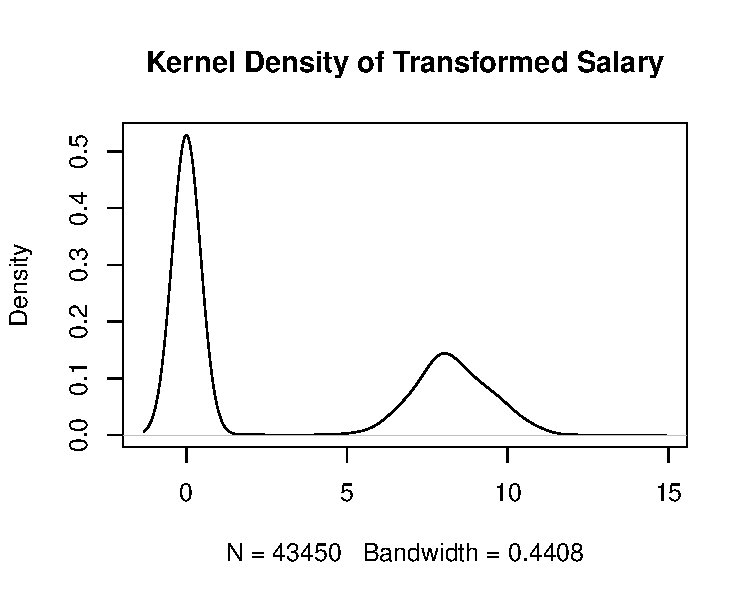
\includegraphics{MLPDF_files/figure-latex/unnamed-chunk-4-1} \end{center}

\hypertarget{training-and-testing-sets}{%
\subsection{Training and Testing Sets}\label{training-and-testing-sets}}

The data were split into two subsamples -- a training and a testing set.
In accordance to Boehmke \& Greenwell (2020), 70\% of the data were
allocated to the training set, and the remaining 30\% to the testing
set. The sample selection was stratified based on the dependent
variable. The tables below illustrates the summary statistics of the
salary variables in Rand terms in the training and testing sets. The
stratification ensures that the observations in the subsamples follow
similar salary distributions.

\begin{table}

\caption{\label{tab:unnamed-chunk-5}Training Set}
\centering
\begin{tabular}[t]{llllllll}
\toprule
Variable & N & Mean & Std. Dev. & Min & Pctl. 25 & Pctl. 75 & Max\\
\midrule
newsal & 30414 & 3124.536 & 8459.82 & 0 & 0 & 3000 & 5e+05\\
\bottomrule
\end{tabular}
\end{table}

\begin{table}

\caption{\label{tab:unnamed-chunk-5}Testing Set}
\centering
\begin{tabular}[t]{llllllll}
\toprule
Variable & N & Mean & Std. Dev. & Min & Pctl. 25 & Pctl. 75 & Max\\
\midrule
newsal & 13036 & 3214.186 & 11079.394 & 0 & 0 & 3000 & 810000\\
\bottomrule
\end{tabular}
\end{table}

All regressions were first tested using resampling methods via 10-fold
cross-validation. In addition, the performance of the regularised
regressions was examined on the test data. All models use pre-processing
to scale or center numeric variables and take out any variables that
exhibit little to no variance (Boehmke \& Greenwell, 2020). The results
of these tests are presented in the next section.

\hypertarget{results}{%
\section{Results}\label{results}}

\hypertarget{linear-models}{%
\subsection{Linear Models}\label{linear-models}}

\hypertarget{multivariate-linear-regression}{%
\subsubsection{Multivariate Linear
Regression}\label{multivariate-linear-regression}}

The first model trained is one which regresses all the possible
dependent variables on the transformed monthly salary. As previously
mentioned, linear models require residuals to be normally distributed.
The density plot below, however, illustrates that the kurtosis of the
residuals is likely too small.

\begin{center}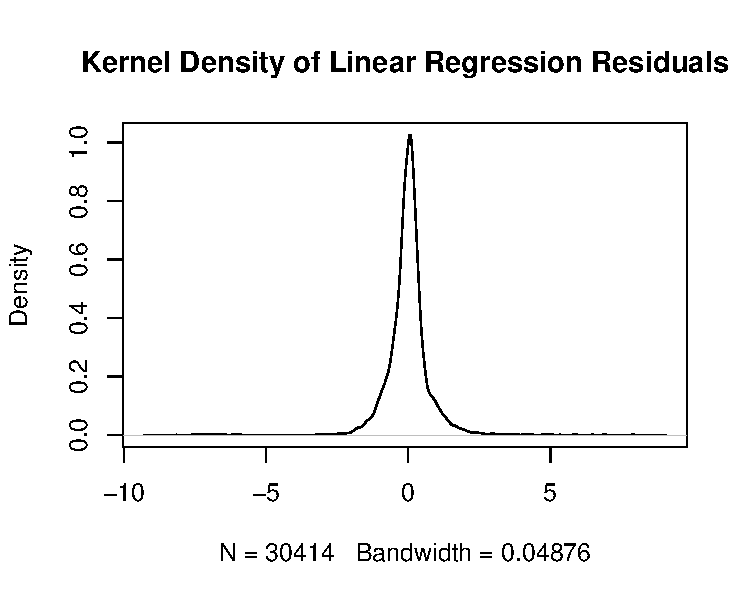
\includegraphics{MLPDF_files/figure-latex/unnamed-chunk-7-1} \end{center}

After resampling, the RMSE of the multivariate linear model is
0.8424206. The R-squared is 0.9586733, implying that the model is
explaining 95\% of the variance in the data. This high R-squared is
likely, however, simply due to the large amount of features added.
Before pre-processing was used to remove 44 near-zero variance
variables, 49 coefficients were undefined by this model, due to
variables exhibiting perfect multicollinearity (Statology, 2021). This
implies that although much of the variance is explained, there is a need
for high correlation between independent variables to be dealt with.

\hypertarget{principal-component-regression}{%
\subsubsection{Principal Component
Regression}\label{principal-component-regression}}

A principal component regression is a form of linear regression that
reduces correlated dimensions before the model is fitted (Boehmke \&
Greenwell, 2020). It follows a two step procedure where highly
correlated features are grouped together and represented in a regression
by other uncorrelated variables, or principal components (Boehmke \&
Greenwell, 2020). This method can improve predictions of the
multivariate linear regression by controlling for multicollinearity
(Boehmke \& Greenwell, 2020). The results of the multivariate linear
regression show that the data used in this paper have many variables
that contain very similar information, such as a feature indicating
whether the household receives a social grant, and another indicating
whether each individual is a recipient. Principal component regression
does not, however, choose principal components based on importance in
predicting the outcome variable. As such, variables included in this
regression may not hold as much predictive power as those in the
multivariate linear model.

\begin{center}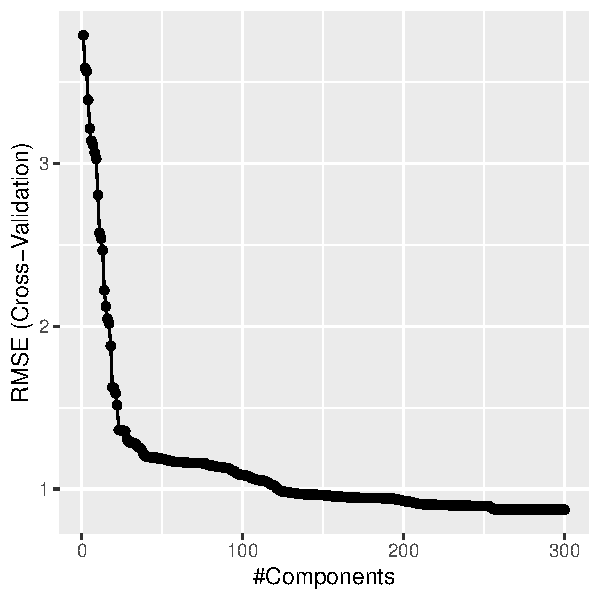
\includegraphics{MLPDF_files/figure-latex/unnamed-chunk-8-1} \end{center}

The principal component regression used in this paper creates 300
principal components, making it computationally inefficient. As can be
seen in the graph below, there is already a large drop in the RMSE after
the use of approximately 25 principal components. The amount of
principal components that produces the lowest RMSE, however, is 299. The
RMSE at this point is 0.8800451, implying that it models the data better
than the previous model. The R-squared is 0.9549784. This illustrates
that a similar amount of variance can be explained by this model as in
the multivariate linear regression model.

\hypertarget{partial-least-squares}{%
\subsubsection{Partial Least Squares}\label{partial-least-squares}}

A partial least squares can build on the faults of principal component
regressions by using the outcome variable to aid in the creation of
components to represent the correlated predictors. This often results in
much higher predictive capabilities (Boehmke \& Greenwell, 2020).

\begin{center}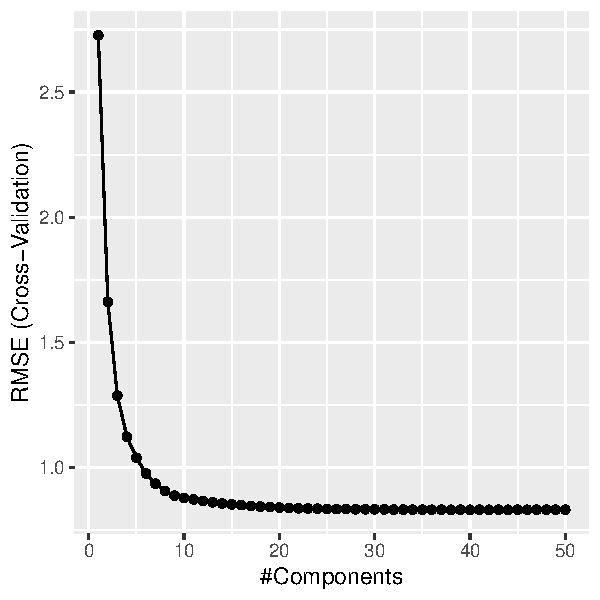
\includegraphics{MLPDF_files/figure-latex/unnamed-chunk-9-1} \end{center}

The partial least squares model creates 50 principal components. While
the above graph shows that there is a significant drop in the RMSE score
after the use of just one principal component, the lowest RMSE
(0.8375993) occurs after the use of 40 components. Therefore, this model
uses less principal components than the principal component regression
and has a slightly lower RMSE than both the previous models. The
R-squared of this model on the training data is similar at 0.9591904.

\hypertarget{regularised-models}{%
\subsection{Regularised Models}\label{regularised-models}}

As is explained above, there are linear models that aim to solve some of
the problems that arise from having many features in a data set.
However, when there are a very high number of variables, linear models
can overfit the data (Boehmke \& Greenwell, 2020). Regularised models
offer techniques to constrain some of the variables, so as to improve
the predictive capabilities on new data. Due to the large number of
features in the GHS 2016 data, a regularised regression is expected to
have more accurate predictions. Both types of regularised regressions
used in this paper make use of a tuning parameter \(\lambda\). As
\(\lambda\) increases, coefficients are pushed closer to zero.

\hypertarget{ridge-regression}{%
\subsubsection{Ridge Regression}\label{ridge-regression}}

A ridge regression constrains coefficients in the model by forcing them
closer to zero as the tuning parameter increases (Boehmke \& Greenwell,
2020). This type of model does not, however, reduce any parameters fully
to zero. This helps to deal with features of low importance, as well as
forcing those that are highly correlated closer to each other.

\begin{center}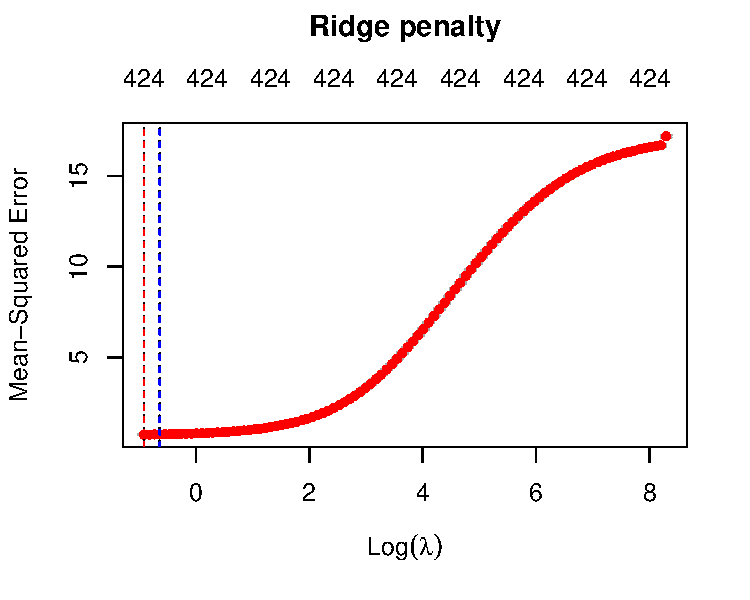
\includegraphics{MLPDF_files/figure-latex/unnamed-chunk-10-1} \end{center}

The optimal tuning parameter for this model is determined by
cross-validation (Boehmke \& Greenwell, 2020). The graph above
illustrates that \(\lambda\) increases, the mean-squared error of this
model on the training data increases. The \(\lambda\) that generates the
lowest mean-squared error for this model is illustrated by the red line,
and is 0.3991006. At this point, the mean-squared error is 0.7497738.
The blue line represents another possible \(\lambda\) value within one
standard deviation away from the red line (Boehmke \& Greenwell, 2020).
When applied to the testing data, the RMSE of the ridge regression
becomes 0.8402423. This implies that the model slightly overfits on the
training data. The R-squared of the ridge regression on the test data is
0.9587792, indicating that it explains approximately 96\% of the
variance in the testing data.

\hypertarget{lasso-regression}{%
\subsubsection{Lasso Regression}\label{lasso-regression}}

A lasso regression model is the same as a ridge regression, but is able
to push coefficients all the way to zero. Not only does this allow for
less important features' impacts to be dampened, but it allows for them
to be removed from the model. Such a model will be helpful to predict
South African salaries, as it will allow for large survey data sets to
become narrower. As a data set becomes narrower, necessary model
assumptions are less likely to be violated (Boehmke \& Greenwell, 2020).

\begin{center}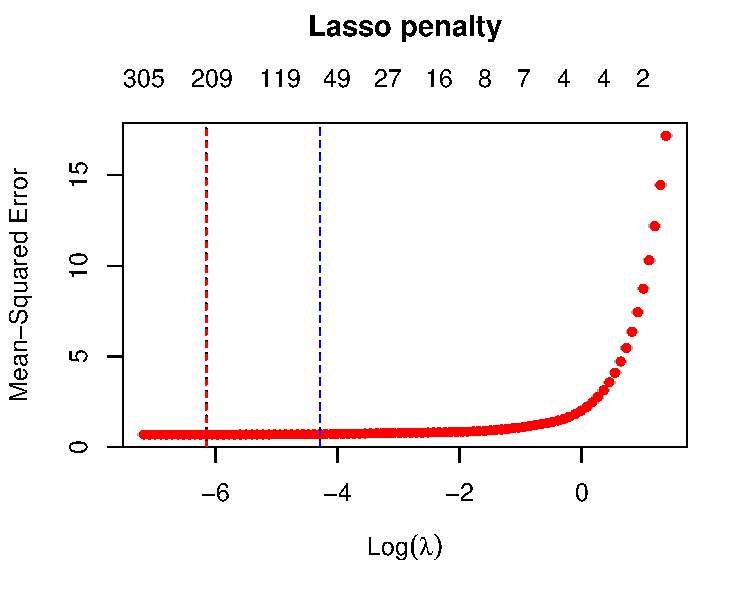
\includegraphics{MLPDF_files/figure-latex/unnamed-chunk-11-1} \end{center}

As is shown by the red line, the lasso regression produces a slightly
lower minimum RMSE (0.8356222) than the ridge regression on the training
data. While the ridge regression uses 424 variables, this model uses
only 233. The blue line illustrates that a similar minimum RMSE
(0.85088806549) can be achieved by using only 70 features. When the
model is applied to the testing data, it achieves a minimum RMSE of
0.8081423. This implies that the model fits the testing data slightly
better than the training data.

\hypertarget{discussion}{%
\section{Discussion}\label{discussion}}

A comparison of RMSE scores shows that all the methods used in this
paper modelled the training data with a similar amount of error, with
the lasso regression scoring the lowest minimum RMSE, and the principal
component regression scoring the highest. This implies that the lasso
regression model predicts South African salaries most accurately. The
table below presents the RMSE values for each model, as well as the RMSE
in Rand terms calculated in the following way:
\[ exp(RMSE_{transformed})-1\] The models all have very similar
R-squared values as well. As mentioned previously, R-squared often
increases simply based on a large amount of features controlled for. The
lasso regression, however, scores a marginally higher R-squared than the
other models and uses significantly fewer features.

\begin{center}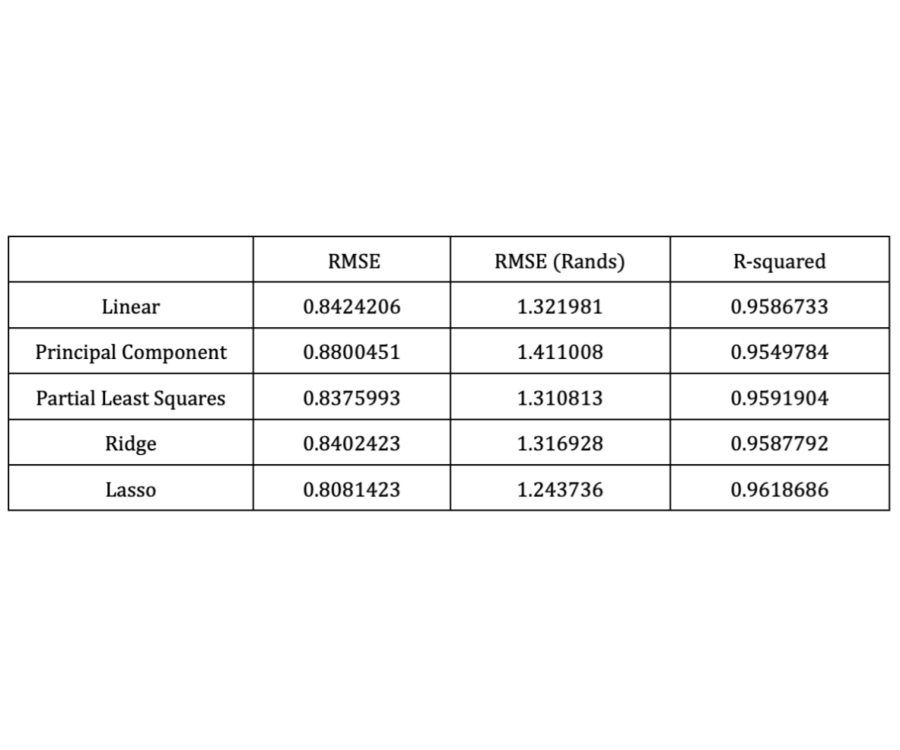
\includegraphics{MLPDF_files/figure-latex/unnamed-chunk-14-1} \end{center}

\hypertarget{coefficients}{%
\subsection{Coefficients}\label{coefficients}}

An important part of economic analysis in the South African context is
determining which factors impact income levels. The graphs below
illustrate the top 10 coefficients that the three linear models deemed
most impactful on the dependent variable. The top graph shows those of
the multivariate linear regression, the middle provides those of the
principal component regression, and the bottom graph illustrates the top
10 coefficients of the partial least squares regression.
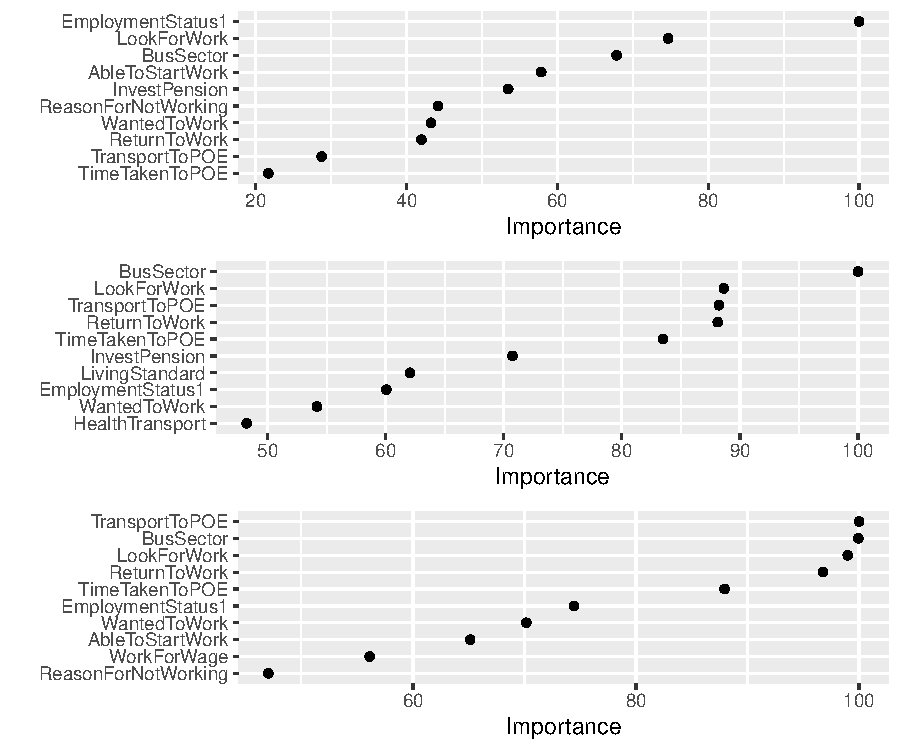
\includegraphics{MLPDF_files/figure-latex/unnamed-chunk-15-1.pdf}

The next two graphs illustrate the same information for the regularised
regressions. The top graph shows that of the ridge regression, and the
bottom graph shows that of the lasso regression.

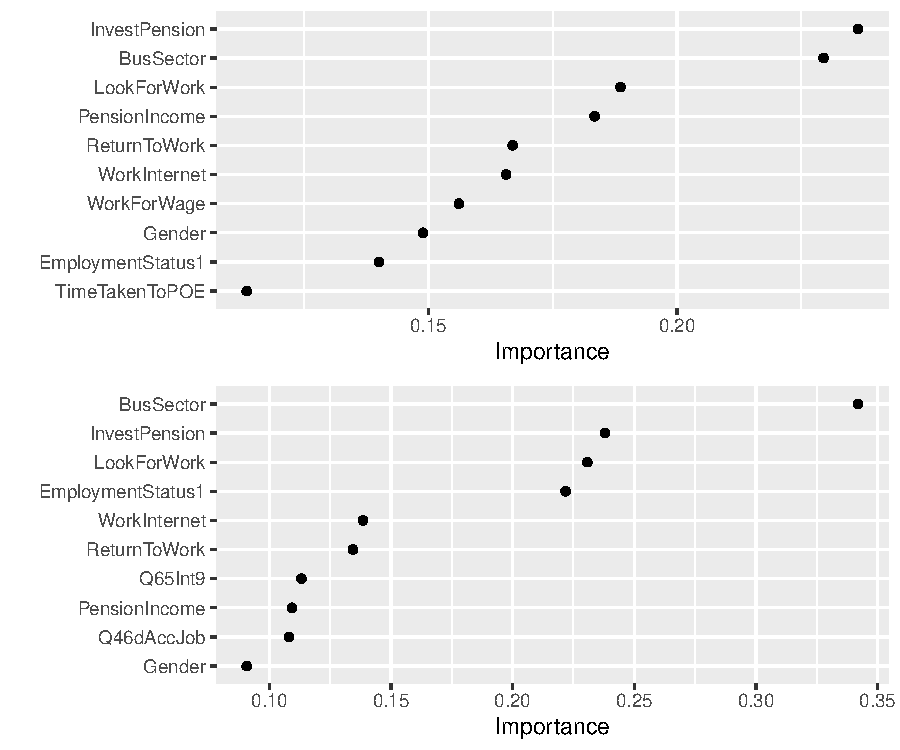
\includegraphics{MLPDF_files/figure-latex/unnamed-chunk-16-1.pdf}

The graphs illustrate that the five models deem similar features to be
in the top 10 most influential to South African salaries. Working in the
business sector and looking for work are within the top three
coefficients of every model. The principal component and partial least
squares regressions both deem that someone having access to transport to
their place of employment as vital in predicting their salary, whereas
the regularised regressions instead consider having pension-related
investments as more important.

Deeming such coefficients as important, however, indicate some reverse
causality. It seems more likely that having a pension-related investment
would occur as a result of someone earning a higher salary, rather than
it contributing to the likelihood of salary increasing. The same
argument applies to most of the other variables viewed as important.
Furthermore, in the South African context, a feature such as race would
play a significant role in someone's salary prospects due to largely
wage gaps between race groups. Only the regularised regressions consider
a fixed feature, such as gender, to play a significant role.

\begin{table}

\caption{\label{tab:unnamed-chunk-17}Salary Across Race Groups}
\centering
\begin{tabular}[t]{llllllll}
\toprule
Variable & N & Mean & Std. Dev. & Min & Pctl. 25 & Pctl. 75 & Max\\
\midrule
Race: 1 &  &  &  &  &  &  & \\
newsal & 36187 & 2360.928 & 6856.74 & 0 & 0 & 2400 & 5e+05\\
Race: 2 &  &  &  &  &  &  & \\
newsal & 4168 & 3159.4 & 8533.466 & 0 & 0 & 3310 & 353500\\
Race: 3 &  &  &  &  &  &  & \\
\addlinespace
newsal & 826 & 8206.195 & 15776.561 & 0 & 0 & 10000 & 258000\\
Race: 4 &  &  &  &  &  &  & \\
newsal & 2269 & 13903.997 & 23576.341 & 0 & 0 & 22139 & 810000\\
\bottomrule
\end{tabular}
\end{table}

In the table above, the numbers one to four indicate race groups: ``1''
shows the statistics for Black South Africans, ``2'' for Coloured South
Africans, ``3'' for Indian or Asian South Africans, and ``4'' for White
South Africans. It illustrates that race is likely not deemed as
important in these regressions, as the GHS 2016 data reports similar
income distributions across race groups. As previously mentioned, this
is not representative of the South African income distribution.

\hypertarget{conclusion}{%
\section{Conclusion}\label{conclusion}}

South African survey data typically contains a large number of features.
In order to draw sound statistical conclusions regarding important
economic topics, such as income, accurate modelling is required. This
paper compared the performance of five machine learning models at
predicting South African incomes. By analysing RMSE and R-squared
scores, it was determined that the lasso regression model performed
marginally better than the other models. In addition, the lasso model
narrows the GHS 2016 data set to only 233 variables. The coefficients
that the models deem as important, however, highlight that the models do
not account for reverse causality. A limitation of this study is that
the dependent variable of choice, monthly salary, is not representative
of the South African context.

\hfill

\newpage

\hypertarget{references}{%
\section*{References}\label{references}}
\addcontentsline{toc}{section}{References}

Boehmke, B. \& Greenwell, B. 2020. \emph{Hands-On Machine Learning with
R}. CRC Press.

Kim, B. 2015. \emph{Should I transform my variables to make them
normally distributed?} {[}Online{]}. Available:
\url{https://data.library.virginia.edu/normality-assumption/} {[}2022,
July{]}.

\bibliography{Tex/ref}





\end{document}
